\documentclass[12pt,a4paper]{report}

\usepackage[T1]{fontenc}
\usepackage[utf8]{inputenc}
\usepackage[english,brazil]{babel}
\usepackage{hyphenat}
\usepackage{indentfirst}
\usepackage{amssymb}
\usepackage{amsmath}
\usepackage{graphicx}
\usepackage{float}
\graphicspath{ {images/} }
\usepackage[backend=biber]{biblatex}
\usepackage{csquotes}
\addbibresource{bibliography.bib}
\usepackage{caption}
\usepackage[hidelinks]{hyperref}
\usepackage{tocloft}
\usepackage{lmodern}
\usepackage{color}
\usepackage[left=3cm,top=3cm,right=2cm,bottom=2cm]{geometry}
\usepackage{fancyhdr}
	\pagestyle{fancy}
	\pagestyle{fancyplain}
	\fancyhf{}
	\rhead{\footnotesize{\thepage}} 
	\renewcommand{\headrulewidth}{0pt}
	\renewcommand{\footrulewidth}{0pt}
\usepackage{bookmark}
\usepackage[bottom]{footmisc}
\usepackage{microtype}
\usepackage{ragged2e}
\usepackage{setspace} 
\usepackage{epigraph}

\newcommand{\I}{{\mathrm{i}\mkern1mu}}
\newcommand{\euler}{{\mathrm{e}\mkern1mu}}

\title{Desenvolvimento de uma plataforma interativa de processamento de sinais}
\author{Mateus Fuga Osmarin}
\date{2021-05-07}

\begin{document}

\pdfbookmark[1]{CAPA}{CAPA}
\begin{minipage}{0.2\linewidth}
  \centering
  
\includegraphics[scale=0.3]{images/uem}
\end{minipage}
\begin{minipage}{0.79\linewidth}
  {
    \centering
    \doublespacing
    \bf
     
    UNIVERSIDADE ESTADUAL DE MARINGÁ\\
    DEPARTAMENTO DE ENGENHARIA QUÍMICA\\
    ENGENHARIA ELÉTRICA\\
  }
\end{minipage}\\[4.54cm]

\center
{
  \bf
  \onehalfspacing
  MATEUS FUGA OSMARIN\\[4.54cm]

  DESENVOLVIMENTO DE UMA PLATAFORMA INTERATIVA DE PROCESSAMENTO DE SINAIS\\[4.54cm]


  TRABALHO DE CONCLUSÃO DE CURSO\\[4.54cm]


  {
    \bf
    MARINGÁ\\
    2021
  }
}
\thispagestyle{empty}
\clearpage


\pdfbookmark[1]{FOLHA DE ROSTO}{FOLHA DE ROSTO}
\begin{figure}[H]
\centering

\includegraphics[scale=0.5]{images/uem_escrito}\\[2.978cm]
\end{figure}
{
  \bf
  {
    MATEUS FUGA OSMARIN\\[2.978cm]

    DESENVOLVIMENTO DE UMA PLATAFORMA INTERATIVA DE PROCESSAMENTO DE SINAIS
  }\\[2.978cm]
}

\begin{minipage}{0.49\linewidth}
  
\includegraphics[scale=0.01]{images/branco} 
\end{minipage}
\begin{minipage}{0.5\linewidth}
{
  \justifying 
  Trabalho de Conclusão de Curso apresentado ao Departamento de Engenharia Química da Universidade Estadual de
  Maringá, como requisito parcial para a obtenção do título de Engenheiro Eletricista.
}\\
\end{minipage}\\[2.978cm]

{
  \center
  Orientador: Prof. Dr. Rafael Krummenauer\\[2.978cm]

  {
    \bf
    Maringá\\
    2021
  }
}

\thispagestyle{empty}
\clearpage

\pdfbookmark[1]{FOLHA DE APROVAÇÃO}{FOLHA DE APROVACAO}
\center

MATEUS FUGA OSMARIN\\[1.86cm]

\textbf{DESENVOLVIMENTO DE UMA PLATAFORMA INTERATIVA DE PROCESSAMENTO DE SINAIS}\\[1.86cm]


\begin{minipage}{0.49\linewidth}

\includegraphics[scale=0.01]{images/branco} 
\end{minipage}
\begin{minipage}{0.5\linewidth}
  {
    \justifying 
    Relatório final apresentado à Universidade Estadual de Maringá como parte das exigências para a obtenção do
    título de Engenheiro Eletricista.
  }\\[1.86cm]

  Maringá, 07 de maio de 2021.\\[1.86cm]
\end{minipage}

{
  \center BANCA EXAMINADORA\\[2.41cm]
}



\rule [0cm]{10cm}{0.1pt}\\
Prof. Dr. Rafael Krummenauer\\
Orientador(a)\\[2.41cm]

\thispagestyle{empty}
\clearpage

\pdfbookmark[1]{DEDICATÓRIA}{DEDICATORIA}
\begin{minipage}{0.9\linewidth}
  
\includegraphics[scale=0.01]{images/branco} 
\end{minipage}\\[21cm]

\begin{minipage}{0.59\linewidth}
  
\includegraphics[scale=0.01]{images/branco} 
\end{minipage}
\begin{minipage}{0.4\linewidth}

\end{minipage}\\[18cm]


\thispagestyle{empty}
\clearpage

\pdfbookmark[1]{AGRADECIMENTOS}{AGRADECIMENTOS}
{
  \center \Large \bf AGRADECIMENTOS
}\\[1cm]

\justifying



\thispagestyle{empty}
\clearpage

\pdfbookmark[1]{EPÍGRAFE}{EPIGRAFE}
\begin{minipage}{0.49\linewidth}
  
\includegraphics[scale=0.01]{images/branco} 
\end{minipage}\\[18cm]

\thispagestyle{empty}
\clearpage

\pdfbookmark[1]{RESUMO}{RESUMO}
\begin{abstract}
  Este trabalho trata do desenvolvimento de uma plataforma interativa de processamento de sinais.
  A partir de uma interface gráfica, é possível realizar o projeto de filtros digitais tanto do tipo
  IIR quanto FIR, utilizando técnicas clássicas da literatura. O sistema busca endereçar a dificuldade
  de visualização no aprendizado do tópico de processamento de sinais, fazendo-se uma ferramenta didática
  alternativa.

  \textbf{Palavras-chave}: Processamento de sinais. Projeto de filtros digitais. Visualização. Python.
\end{abstract}

\pdfbookmark[1]{ABSTRACT}{ABSTRACT}
\begin{otherlanguage}{english}
  \begin{abstract}
    This paper addresses the development of an interactive signal processing platform. By means of a graphical
    user interface, it is possible to design both IIR and FIR filters, using classic techniques. The system
    aims to deal with the visualization issues in the learning of signal processing topic, being an alternative
    didatic tool.

    \textbf{Keywords}: Signal processing. Digital filter design. Visualization. Python.
  \end{abstract}
\end{otherlanguage}

{
  \pdfbookmark[1]{LISTA DE FIGURAS}{LISTA DE FIGURAS}
  \center
  \listoffigures
  \pagestyle{empty}
  \clearpage
}

{
  \pdfbookmark[1]{SUMÁRIO}{SUMARIO}
  \center
  \tableofcontents
  \thispagestyle{empty}
  \clearpage
}

\thispagestyle{empty}
\clearpage
\onehalfspacing

\chapter{Introdução}
  A disciplina de processamento de sinais é uma área ampla que permite entender e tratar matematicamente
  sinais, transformando-os segundo as necessidades envolvidas na sua aplicação. Majoritariamente, encontra-se
  no dia-a-dia sinais de natureza contínua no tempo, como a temperatura de um corpo, o som de um instrumento
  musical ou a velocidade de um automóvel. Ainda, existem sinais de natureza inerentemente discreta no tempo,
  como é o caso do preço de uma ação, as temperaturas máxima e mínima diárias de uma cidade ou o número diário
  de novos casos de COVID-19. Entretanto, é importante ressaltar que mesmo sinais de natureza contínua  podem
  ser tratados de forma discreta por meio de procedimentos de amostragem adequados. Dessa forma, o processamento
  digital de sinais pode ser aplicado a uma infinidade de casos.

  Diante da generalidade envolvida, tem-se também um nível de abstração elevado no formalismo matemático que
  fundamenta a disciplina, o que resulta em dificuldades no aprendizado dessa importante área. Nesse sentido,
  a utilização de ferramentas como o Filter Designer do MATLAB traz benefícios tanto de produtividade para
  profissionais da área como facilitam o aprendizado para estudantes do tópico, por abordar de forma visual e
  intuitiva o projeto de filtros digitais. Utilizando esse tipo de ferramenta, pode-se variar parâmetros de
  projeto e visualizar o comportamento dos sistemas projetados de forma eficiente e facilitada, com gráficos que
  exibem as principais características do processo. Contudo, o MATLAB se trata de um software pago e, não
  obstante, tem-se observado um aumento crescente no interesse pela linguagem de programação Python por
  estudantes e profissionais da área da ciência e tecnologia, dada a grande quantidade de bibliotecas disponíveis
  para todo tipo de problemas.

\chapter{Objetivos}
\section{Objetivos gerais}
  O presente trabalho tem como objetivo o desenvolvimento de um software livre para projeto de filtros digitais
  utilizando a linguagem de programação Python, construindo uma interface gráfica amigável em GTK para aumento
  de produtividade e facilitar o aprendizado na área de processamento de sinais, contando com uma revisão de
  conceitos importantes a servir como referência para utilização do sistema.

\section{Objetivos específicos}
Os objetivos específicos deste trabalho consistem no desenvolvimento de uma aplicação com interface gráfica que
  \begin{itemize}
    \item possibilite projetar filtros FIR e IIR utilizando técnicas clássicas da literatura;
    \item permita visualizar as principais características dos filtros projetados, como resposta em frequência
      (amplitude e fase), localização de polos e zeros no plano complexo e resposta ao impulso;
    \item tenha a opção de exportar o filtro projetado para que seja possível utilizá-lo externamente.
  \end{itemize}

\chapter{Referenciais teóricos}
\section{Sinais}
  Em essência, um sinal é algo que contém alguma informação, geralmente sobre o estado de um sistema físico
  \cite{oppenheim}. Podemos definir matematicamente um sinal como sendo uma função, de uma ou mais variáveis
  independentes. A natureza dessas variáveis é diversa, sendo o tempo e o espaço as mais usuais. O som é um
  exemplo de sinal temporal, enquanto a temperatura em uma sala ao longo do dia se refere a um sinal espacial e
  temporal. No decorrer deste trabalho, serão considerados sinais de uma variável, sendo tomada como temporal
  por convenção, mas a teoria é igualmente válida para outros domínios.

  Um sinal contínuo no tempo é definido como sendo uma função do tempo definida para todos os instantes:
  \begin{equation}
    x = x(t), t \in \mathbb{R}
  \end{equation}
  A figura \ref{fig:continuous} mostra um exemplo de sinal contínuo no tempo.
  \begin{figure}[H]
    \caption{Sinal contínuo no tempo}
    \centering
    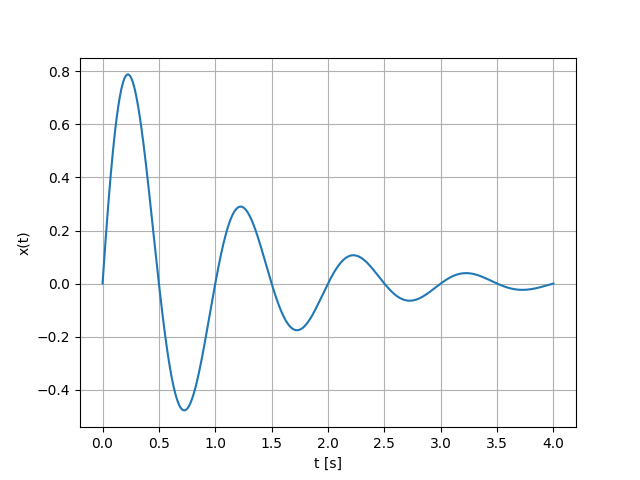
\includegraphics[width=0.75\textwidth]{continuous}
    \label{fig:continuous}
    \caption*{Fonte: Autoria própria}
  \end{figure}

  Um sinal discreto no tempo, por outro lado, é definido como uma sequência numérica:
  \begin{equation}
    x = x[n], n \in \mathbb{Z}
  \end{equation}

  Para tratar discretamente sinais contínuos no tempo, pode-se amostrar o sinal contínuo em intervalos de tempo
  igualmente espaçados:
  \begin{equation}
    x_d[n] = x_a(n T_s)
  \end{equation}
  onde $x_d$ é a versão discretizada do sinal analógico $x_a$ e $T_s$ representa o período de amostragem.
  A figura \ref{fig:discrete} mostra o sinal da figura \ref{fig:continuous} discretizado.
  \begin{figure}[H]
    \caption{Sinal discreto no tempo}
    \centering
    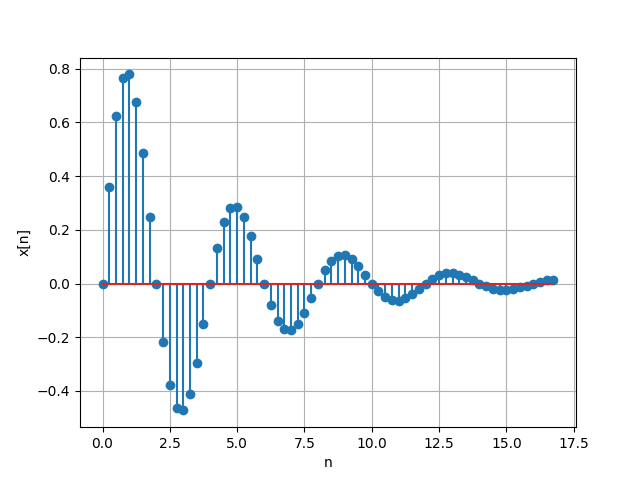
\includegraphics[width=0.75\textwidth]{discrete}
    \label{fig:discrete}
    \caption*{Fonte: Autoria própria}
  \end{figure}

  Para discretizar um sinal adequadamente, sem perda de informação e sem gerar distorção (\textit{aliasing}), o
  teorema da amostragem de Nyquist-Shannon \cite{lathi} afirma que a amostragem deve ser feita a uma taxa $f_s$
  superior ao dobro da maior frequência no espectro do sinal $f_m$, ou seja
  \begin{equation}
    f_s > 2 f_m
  \end{equation}

  De forma equivalente, no domínio do tempo, tem-se que o período de amostragem $T_s$ deve ser
  \begin{equation}
    T_s  < \frac{1}{2 f_m}
  \end{equation}

  Dentre os sinais existentes, o impulso unitário ou delta de Dirac, é um dos mais importantes. Este sinal é
  definido, no caso contínuo, como:
  \begin{equation}
    \delta(t) =
      \left
      \{
      \begin{array}{rcl}
        0 & \mbox{para} & t \neq 0 \\
        \infty & \mbox{para} & t = 0
      \end{array}
      \right.
  \end{equation}
  satisfazendo a restrição
  \begin{equation}
    \int_{-\infty}^{+\infty} \delta(t) dt = 1
  \end{equation}

  Uma propriedade notória do impulso unitário é que
  \begin{equation}
    \int_{-\infty}^{+\infty} f(t) \delta(t-t_0) dt = f(t_0)
  \end{equation}
  sendo conhecida como propriedade da amostragem.

  No caso discreto, o impulso unitário é definido como:
  \begin{equation}
    \delta[n] =
      \left
      \{
      \begin{array}{rcl}
        0 & \mbox{para} & n \neq 0 \\
        1 & \mbox{para} & n = 0
      \end{array}
      \right.
  \end{equation}

  A propriedade da amostragem para o caso discreto é expressa como:
  \begin{equation}
    \sum_{n = -\infty}^{+\infty} x[n] \delta[n-n_0] = x[n_0]
  \end{equation}

\section{Transformadas de Fourier, Laplace e Z}
  Até aqui, os sinais foram descritos no domínio do tempo. É possível, no entanto, representar sinais no
  domínio da frequência através das transformações conhecidas como transformada de Fourier, transformada de
  Laplace e transformada Z. O princípio de partida é a série de Fourier, que possibilita a representação de uma
  função T-periódica como uma série de senos e cossenos ou, equivalentemente, exponenciais complexas.

  A série de Fourier é definida como:
  \begin{equation}
    x_N(t) = \sum_{n = -N}^{+N} c_n \euler^{\I \frac{2 \pi}{T} n t}
  \end{equation}
  onde
  \begin{equation}
    c_n = \frac{1}{T} \int_T x(t) \euler^{-\I \frac{2 \pi}{T} n t} dt
  \end{equation}
  são os coeficientes da série, e N é teoricamente infinito. A figura \ref{fig:fourier} mostra a expansão
  em série de Fourier do retângulo unitário para diferentes valores de N.
  \begin{figure}[H]
    \caption{Expansão em série de Fourier do retângulo unitário}
    \centering
    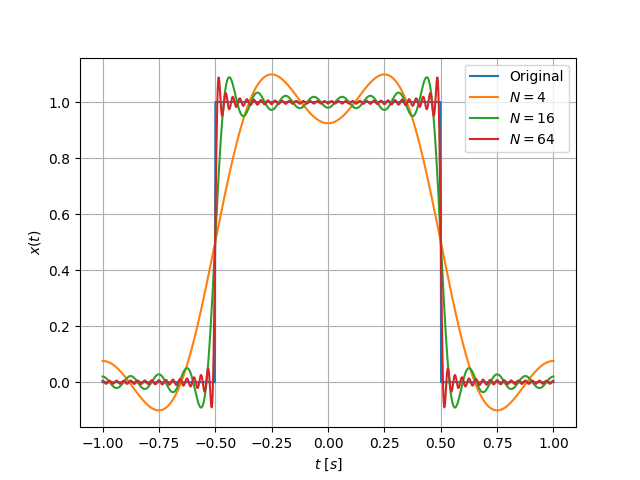
\includegraphics[width=0.75\textwidth]{fourier_series}
    \label{fig:fourier}
    \caption*{Fonte: Autoria própria}
  \end{figure}

  Para funções não-periódicas, generaliza-se a série de Fourier considerando o período como sendo infinito.
  No caso limite, tem-se:
  \begin{equation}
    x(t) = \int_{-\infty}^{+\infty} \widehat{x}(f) \euler^{\I 2 \pi f t} df
  \end{equation}
  onde
  \begin{equation}
    \widehat{x}(f) = \mathcal{F}\{x(t)\}(f) = \int_{-\infty}^{+\infty} x(t) \euler^{-\I 2 \pi f t} dt
  \end{equation}
  e $\widehat{x}(f)$ é conhecida como a transformada de Fourier de $x(t)$. Segundo esta definição, $f$ tem
  unidades de $hertz$. A figura \ref{fig:fourier_transform} mostra a transformada de Fourier do retângulo
  unitário.
  \begin{figure}[H]
    \caption{Transformada de Fourier do retângulo unitário}
    \centering
    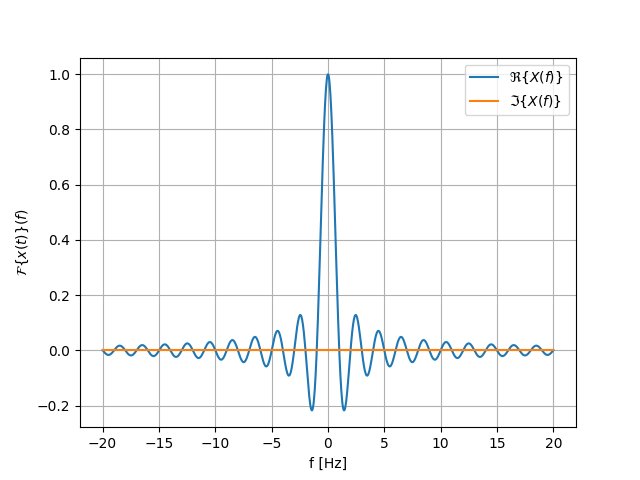
\includegraphics[width=0.75\textwidth]{fourier_transform}
    \label{fig:fourier_transform}
    \caption*{Fonte: Autoria própria}
  \end{figure}

  Ao amostrar um sinal com um período de amostragem $T$ por meio de um pente de Dirac
  \begin{equation}
    \begin{split}
      x_T(t) = &\quad x(t) \sum_{n = -\infty}^{+\infty} \delta(t - n T) \\
      = &\quad \sum_{n = -\infty}^{+\infty} x(n T) \delta(t - n T) \\
      = &\quad \sum_{n = -\infty}^{+\infty} x[n] \delta(t - n T)
    \end{split}
    \label{eq:dirac_comb}
  \end{equation}
  e aplicar a transformada de Fourier, tem-se
  \begin{equation}
    \begin{split}
      \widehat{x}_T(f) = &\quad \int_{-\infty}^{+\infty} \sum_{n = -\infty}^{+\infty}
                                x[n] \delta(t - n T) \euler^{-\I 2 \pi f t} dt
      \\ = &\quad \sum_{n = -\infty}^{\infty} x[n] \int_{-\infty}^{+\infty}
                                \delta(t - n T) \euler^{-\I 2 \pi f t} dt
      \\ = &\quad \sum_{n = -\infty}^{+\infty} x[n] \euler^{-\I 2 \pi f n T}
    \end{split}
  \end{equation}
  ao que se obtém a chamada transformada de tempo discreto de Fourier. Para obter o sinal original, a
  transformada de tempo discreto de Fourier inversa é:
  \begin{equation}
    x[n] = T \int_{1/T} \widehat{x}_T(f) \euler^{\I 2 \pi f n T} df
  \end{equation}

  A figura \ref{fig:discrete_time_fourier_transform} mostra a transformada de tempo discreto de Fourier do
  retângulo unitário.
  \begin{figure}[H]
    \caption{Transformada de tempo discreto de Fourier do retângulo unitário}
    \centering
    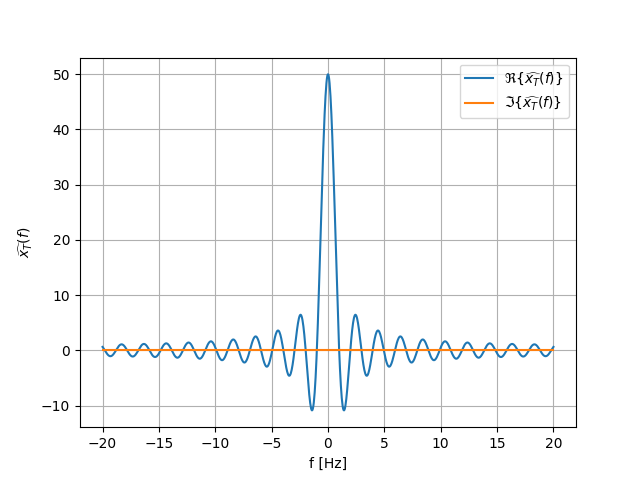
\includegraphics[width=0.75\textwidth]{discrete_time_fourier_transform}
    \label{fig:discrete_time_fourier_transform}
    \caption*{Fonte: Autoria própria}
  \end{figure}
  Nesse caso, a discretização acontece no domínio do tempo, mas a frequência ainda é contínua. Discretizando a
  transformada de tempo discreto de Fourier para $N$ amostras de um ciclo, obtém-se:
  \begin{equation}
    \begin{split}
      X[k] = &\quad \widehat{x}_T\left(\frac{k}{N T}\right)
      \\ &\quad = \sum_{n = -\infty}^{+\infty} x[n] \euler^{-\I 2 \pi \frac{k}{N T} n T}
      \\ &\quad = \sum_{n = -\infty}^{+\infty} x[n] \euler^{-\I 2 \pi \frac{k}{N} n}
    \end{split}
  \end{equation}
  o que define a transformada discreta de Fourier. Para obter o sinal original, a transformada discreta de
  Fourier inversa é:
  \begin{equation}
    x[n] = \frac{1}{N} \sum_{k = -\infty}^{+\infty} X[k] \euler^{\I 2 \pi \frac{k}{N} n}
  \end{equation}
  
  A figura \ref{fig:discrete_fourier_transform} mostra a transformada discreta de Fourier do retângulo unitário.
  \begin{figure}[H]
    \caption{Transformada discreta de Fourier do retângulo unitário}
    \centering
    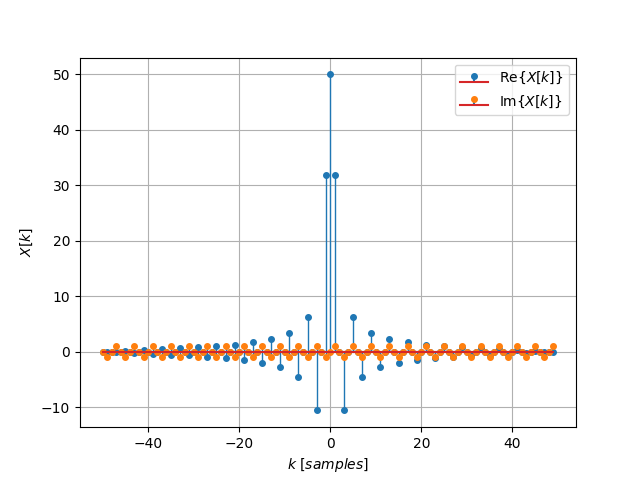
\includegraphics[width=0.75\textwidth]{discrete_fourier_transform}
    \label{fig:discrete_fourier_transform}
    \caption*{Fonte: Autoria própria}
  \end{figure}

  A transformada de Fourier pode ainda ser generalizada ao se considerar uma frequência complexa. O resultado
  é a transformada de Laplace:
  \begin{equation}
    X(s) = \mathcal{L}\{x(t)\}(s) = \int_{-\infty}^{+\infty} x(t) \euler^{-s t} dt
  \end{equation}
  onde
  \begin{equation}
    s = \sigma + \I \omega = \sigma + \I 2 \pi f
  \end{equation}

  A figura \ref{fig:laplace_transform} mostra a transformada de Laplace do retângulo unitário.
  \begin{figure}[H]
    \caption{Transformada de Laplace do retângulo unitário}
    \centering
    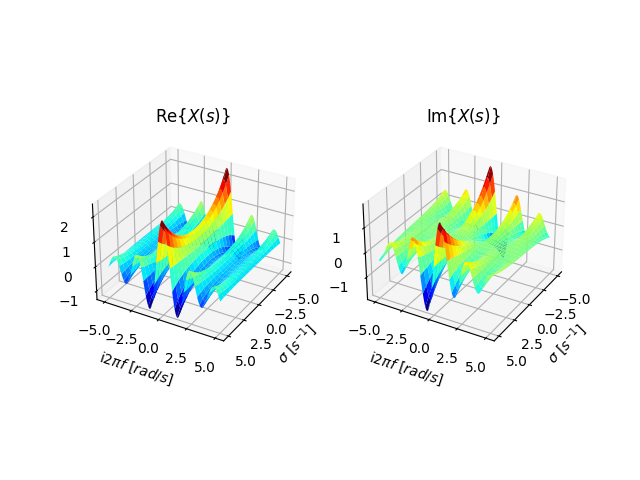
\includegraphics[width=0.75\textwidth]{laplace_transform}
    \label{fig:laplace_transform}
    \caption*{Fonte: Autoria própria}
  \end{figure}

  Nota-se também que a transformada de Laplace pode ser vista como sendo a transformada de Fourier de
  $x(t) \euler^{-\sigma t}$. Para recuperar o sinal original, a transformada de Laplace inversa é:
  \begin{equation}
    x(t) = \mathcal{L}^{-1}\{X(s)\}(t) = \frac{1}{\I 2 \pi} \lim_{T \rightarrow \infty}
    \int_{\gamma - \I T}^{\gamma + \I T} X(s) \euler^{s t} ds
  \end{equation}
  onde $\gamma$ é um número real tal que o caminho de integração esteja na região de convergência de $F(s)$.

  Novamente, amostrando um sinal por meio de um pente de Dirac \eqref{eq:dirac_comb} e aplicando
  a transformada de Laplace, tem-se
  \begin{equation}
    \begin{split}
      X_T(s) = &\quad \int_{-\infty}^{+\infty} \sum_{n = -\infty}^{+\infty} x[n] \delta(t - n T) \euler^{-s t} dt
      \\= &\quad \sum_{n = -\infty}^{+\infty} x[n] \int_{-\infty}^{+\infty} \delta(t - n T) \euler^{-s t} dt
      \\= &\quad \sum_{n = -\infty}^{+\infty} x[n] \euler^{-s n T}
    \end{split}
  \end{equation}
  da qual, ao tomar $z = \euler^{s T}$, obtém-se a transformada Z de um sinal discreto:
  \begin{equation}
    X(z) = \mathcal{Z}\{x[n]\}(z) = \sum_{n = -\infty}^{+\infty} x[n] z^{-n}, z \in \mathbb{C}
  \end{equation}

  Para recuperar o sinal original, a transformada Z inversa é:
  \begin{equation}
    x[n] = \mathcal{Z}^{-1}\{X(z)\}[n] = \frac{1}{\I 2 \pi} \oint_{\mathcal{C}} X(z) z^{n - 1} dz
  \end{equation}
  onde $\mathcal{C}$ é um caminho fechado percorrido no sentido anti-horário, contendo a origem e inteiramente
  na região de convergência de $X(z)$.

\section{Convolução}
  Dados dois sinais, é possível realizar um conjunto de operações sobre os mesmos. Dentre estas, tem-se as bem
  conhecidas operações de soma, subtração, multiplicação, divisão, derivação e integração. Em processamento
  de sinais, uma operação conhecida como convolução é muito utilizada, sendo definida por:
  \begin{equation}
    (f \ast g)(t) = \int_{-\infty}^{+\infty} f(\tau) g(t - \tau) d\tau
  \end{equation}
  para o caso contínuo e
  \begin{equation}
    (f \ast g)[n] = \sum_{k = -\infty}^{+\infty} f[k] g[n - k]
  \end{equation}
  para o caso discreto.

  Uma propriedade importante da convolução é
  \begin{equation}
    \label{eq:continuous_convolution_identity}
    x(t) \ast \delta(t) = \int_{-\infty}^{+\infty} x(\tau) \delta(t - \tau) d\tau = x(t)
  \end{equation}
  para o caso contínuo e
  \begin{equation}
    \label{eq:discrete_convolution_identity}
    x[n] \ast \delta[n] = \sum_{k = -\infty}^{+\infty} x[k] \delta[n - k] = x[n]
  \end{equation}
  para o caso discreto. Esta propriedade exprime o fato de que o impulso unitário corresponde a uma identidade
  para a convolução.

  Ainda, outra propriedade importante da convolução está em sua relação com as transformadas de Fourier, Laplace
  e Z. Tomando a transformada de Laplace como exemplo, tem-se:
  \begin{equation}
    \label{eq:convolution_theorem}
    \begin{split}
      \mathcal{L}\{(f \ast g)(t)\}(s) = &\quad \int_{t = -\infty}^{+\infty} \left[\int_{\tau = -\infty}^{+\infty}
      f(\tau) g(t - \tau) d\tau\right] \euler^{-s t} dt
      \\ = &\quad \int_{\tau = -\infty}^{+\infty} \int_{t = -\infty}^{+\infty}
      f(\tau) g(t - \tau) \euler^{-s t} dt d\tau
      \\ = &\quad \int_{\tau = -\infty}^{+\infty} f(\tau) \int_{t = -\infty}^{+\infty}
      g(t - \tau) \euler^{-s t} dt d\tau
      \\ = &\quad \int_{\tau = -\infty}^{+\infty} f(\tau) \int_{u = -\infty}^{+\infty}
      g(u) \euler^{-s(u+\tau)} du d\tau
      \\ = &\quad \int_{\tau = -\infty}^{+\infty} f(\tau) \euler^{-s \tau} d\tau
      \int_{u = -\infty}^{+\infty} g(u) \euler^{-s u} du
      \\ = &\quad \mathcal{L}\{f(t)\}(s) \mathcal{L}\{g(t)\}(s)
    \end{split}
  \end{equation}
  ou seja, no domínio da frequência a operação de convolução corresponde à multiplicação. A equação
  \ref{eq:convolution_theorem} é conhecida como teorema do convolução.

\section{Sistemas lineares e invariantes no tempo}
  Um sistema é essencialmente algo que mapeia um sinal de entrada em um sinal de saída \cite{diniz}, ou seja:
  \begin{equation}
    y(t) = \mathcal{H}\{x(t)\}
  \end{equation}
  para um sistema analógico e
  \begin{equation}
    y[n] = \mathcal{H}\{x[n]\}
  \end{equation}
  para um sistema discreto, onde $\mathcal{H}\{\cdot\}$ denota o sistema.

  Dentre todos os sistemas possíveis, tem-se classes de sistemas que são interessantes pelas propriedades que
  apresentam. Um sistema linear é um sistema que tem a propriedade:
  \begin{equation}
    \mathcal{H}\{a x_1(t) + b x_2(t)\} = a \mathcal{H}\{x_1(t)\} + b \mathcal{H}\{x_2(t)\}
  \end{equation}
  para o caso contínuo e
  \begin{equation}
    \mathcal{H}\{a x_1[n] + b x_2[n]\} = a \mathcal{H}\{x_1[n]\} + b \mathcal{H}\{x_2[n]\}
  \end{equation}
  para o caso discreto. Sistemas com essa propriedade tem a característica de, por exemplo, ao se dobrar a
  amplitude da entrada, dobrar-se também a amplitude da saída.

  Um sistema invariante no tempo é um sistema que tem a propriedade:
  \begin{equation}
    \mathcal{H}\{x(t)\} = y(t) \Leftrightarrow \mathcal{H}\{x(t - t_0)\} = y(t - t_0)
  \end{equation}
  para o caso contínuo e
  \begin{equation}
    \mathcal{H}\{x[n]\} = y[n] \Leftrightarrow \mathcal{H}\{x[n - n_0]\} = y[n - n_0]
  \end{equation}
  para o caso discreto. Sistemas com essa propriedade tem a característica de ao se atrasar a entrada, atrasar-se
  também a saída pela mesma quantidade.

  Sistemas que são lineares e invariantes no tempo podem ser tratados matemáticamente de forma generalizada como
  se segue. Sendo $\mathcal{H}\{\cdot\}$ um sistema linear e invariante no tempo, e como, de acordo com as
  equações \ref{eq:continuous_convolution_identity} e \ref{eq:discrete_convolution_identity}, sinais podem ser
  representados por uma convolução com o impulso unitário, tem-se
  \begin{equation}
    \label{eq:continuous_system_convolution}
    \begin{split}
      y(t) = &\quad \mathcal{H}\{x(t) \ast \delta(t)\}
      = \mathcal{H}\{\int_{-\infty}^{+\infty} x(\tau) \delta(t - \tau) d\tau\}
      \\ = &\quad \int_{-\infty}^{+\infty} x(\tau) \mathcal{H}\{\delta(t - \tau)\} d\tau
      \\ = &\quad \int_{-\infty}^{+\infty} x(\tau) h(t - \tau) d\tau
      \\ = &\quad x(t) \ast h(t)
    \end{split}
  \end{equation}
  para o caso contínuo e
  \begin{equation}
    \label{eq:discrete_system_convolution}
    \begin{split}
      y[n] = &\quad \mathcal{H}\{x[n] \ast \delta[n]\}
      = \mathcal{H}\{\sum_{k = -\infty}^{+\infty} x[k] \delta[n - k]\}
      \\ = &\quad \sum_{k = -\infty}^{+\infty} x[k] \mathcal{H}\{\delta[n - k]\}
      \\ = &\quad \sum_{k = -\infty}^{+\infty} x[k] h[n - k]
      \\ = &\quad x[n] \ast h[n]
  \end{split}
  \end{equation}
  para o caso discreto. Nas equações \ref{eq:continuous_system_convolution} e
  \ref{eq:discrete_system_convolution}, $h(t)$ e $h[n]$ representam a resposta do sistema a um impulso unitário.
  Assim, um sistema linear e invariante no tempo pode ser descrito totalmente por sua resposta ao impulso.

  No domínio da frequência, o teorema da convolução \ref{eq:convolution_theorem} fornece:
  \begin{equation}
    Y(s) = \mathcal{L}\{x(t) \ast h(t)\} = X(s) H(s)
  \end{equation}
  para um sistema analógico e
  \begin{equation}
    Y(z) = \mathcal{Z}\{x[n] \ast h[n]\} = X(z) H(z)
  \end{equation}
  para um sistema discreto. Chama-se $H(s)$ e $H(z)$ a função de transferência do sistema $\mathcal{H\{\cdot}\}$.
\section{Filtros digitais}
  Em geral, um filtro digital é um sistema discreto cujo objetivo é destacar ou reduzir determinadas
  características de um sinal. Neste trabalho serão abordados filtros digitais lineares e invariantes no tempo.

  Filtros não-recursivos são caracterizados por uma equação de diferenças do tipo:
  \begin{equation}
    y[n] = \sum_{k = 0}^{M} b_k x[n - k]
  \end{equation}
  onde os coeficientes $b_k$ estão diretamente relacionados à resposta ao impulso do sistema, ou seja,
  $b_k = h[k]$. Aplicando a transformada Z, tem-se que a função de transferência do sistema é dada por:
  \begin{equation}
    H(z) = \frac{Y(z)}{X(z)} = \sum_{k = 0}^{M} b_k z^{-k}
  \end{equation}
  Devido ao fato de a resposta ao impulso deste sistema ser de duração finita, filtros não-recursivos são também
  conhecidos como filtros de resposta ao impulso finito (FIR, do inglês \textit{finite impulse response}).

  Filtros recursivos, por outro lado, são caracterizados por uma equação de diferenças do tipo:
  \begin{equation}
    y[n] = \sum_{k = 0}^{M} b_k x[n - k] - \sum_{k = 1}^{N} a_k y[n - k]
  \end{equation}
  Aplicando a transformada Z, tem-se
  \begin{equation}
    Y(z) = \sum_{k = 0}^{M} b_k X(z) z^{-k} - \sum_{k = 1}^{N} a_k Y(z) z^{-k}
  \end{equation}
  de onde, ao se rearranjar, obtem-se
  \begin{equation}
    Y(z) \left( 1 + \sum_{k = 1}^{N} a_k z^{-k} \right) = X(z) \left( \sum_{k = 0}^{M} b_k z^{-k} \right)
  \end{equation}
  ou seja,
  \begin{equation}
    H(z) = \frac{Y(z)}{X(z)} = \frac{\sum_{k = 0}^{M} b_k z^{-k}}{1 + \sum_{k = 1}^{N} a_k z^{-k}}
  \end{equation}
  é a função de transferência do sistema. Filtros recursivos, pelo fato de que a saída do sistema depende de
  saídas passadas, apresentam uma resposta ao impulso de duração infinita, dessa forma são também conhecidos como
  filtros de resposta ao impulso infinito (IIR, do inglês \textit{infinite impulse response}).

  Neste trabalho serão abordados projetos de filtros digitais por métodos de otimização como
  \textit{Least Squares} \cite{selesnick}, o algoritmo de Remez \cite{mcclellan_parks} e a transformação bilinear
  \cite{diniz} aplicada aos clássicos filtros de Butterworth, Chebyshev, Cauer e Bessel.
\chapter{Metodologia}
  O principal objetivo deste trabalho foi o desenvolvimento de uma aplicação com interface gráfica para projeto
  de filtros digitais. Neste capítulo, serão apresentados detalhes sobre a elaboração do software.

  A ferramenta foi desenvolvida em Python 3 \cite{python}, utilizando as bibliotecas GTK \cite{gtk, pygtk}, para
  interface gráfica, NumPy \cite{numpy} para computação numérica eficiente, SciPy \cite{scipy} para projeto dos
  filtros e Matplotlib \cite{matplotlib} para visualização de dados.
  O código foi escrito totalmente pelo autor, de forma modular, facilitando modificações e a inclusão de novas
  funcionalidades, estando disponível publicamente no Github \cite{source_code}. Instruções de instalação estão
  inclusas no README do repositório.

  O programa foi estruturado na seguinte hierarquia:
  \begin{itemize}
    \item \texttt{main.py}, é o módulo principal responsável por montar toda a aplicação,
    \item \texttt{fdatool/utils.py}, apresenta utilitários para conversão entre diferentes unidades de medida de
      frequência (Hz, kHz, MHz e GHz) e amplitude (dB, V e W), bem como uma classe representado eventos que podem
      ocorrer durante a execução do programa, permitindo o registro de callbacks,
    \item \texttt{fdatool/widgets/inputs.py}, constrói os componentes de entrada de dados da aplicação,
      adicionando controle de estado aos mesmos,
    \item \texttt{fdatool/widgets/specs.py}, trata dos componentes de especificações de frequência e amplitude,
    \item \texttt{fdatool/widgets/common.py}, contém componentes gŕaficos recorrentes como botões e componente
      para seleção de ordem dos filtros,
    \item \texttt{fdatool/widgets/figures.py}, onde são construídos os gráficos da aplicação,
    \item \texttt{fdatool/filters/firls.py}, este módulo implementa os filtros FIR utilizando o método Least
      Squares,
    \item \texttt{fdatool/filters/remez.py}, cuja função é o projeto de filtros FIR pelo algoritmo de Remez,
    \item \texttt{fdatool/filters/iir.py}, contém os filtros clássicos que são discretizados pela transformação
      bilinear,
    \item \texttt{fdatool/filters/factory.py}, permite a obtenção de um dos métodos de projeto por meio de uma
      fábrica \cite{gang_of_four}.
  \end{itemize}

  O software foi escrito levando em consideração padrões de projeto \cite{gang_of_four} como \textit{decorator},
  \textit{observer}, \textit{state} e \textit{factory method}, sendo adaptados pelo autor de modo a harmonizar
  com o ecossistema Python.

\chapter{Resultados}
  Neste capítulo será apresentada a aplicação desenvolvida, bem como sua forma de uso. Ainda, será realizado o
  projeto de alguns filtros utilizando a ferramenta construída. Os filtros terão frequência de amostragem de
  44.1 kHz, frequência típica de áudio digital com qualidade de CD.

  A tela inicial do programa é mostrada na figura \ref{fig:home}. O sistema consiste de duas seções: as
  especificações do filtro a ser projetado e os gráficos que mostram os resultados do processo.
  \begin{figure}[H]
    \caption{Tela inicial da ferramenta desenvolvida}
    \centering
    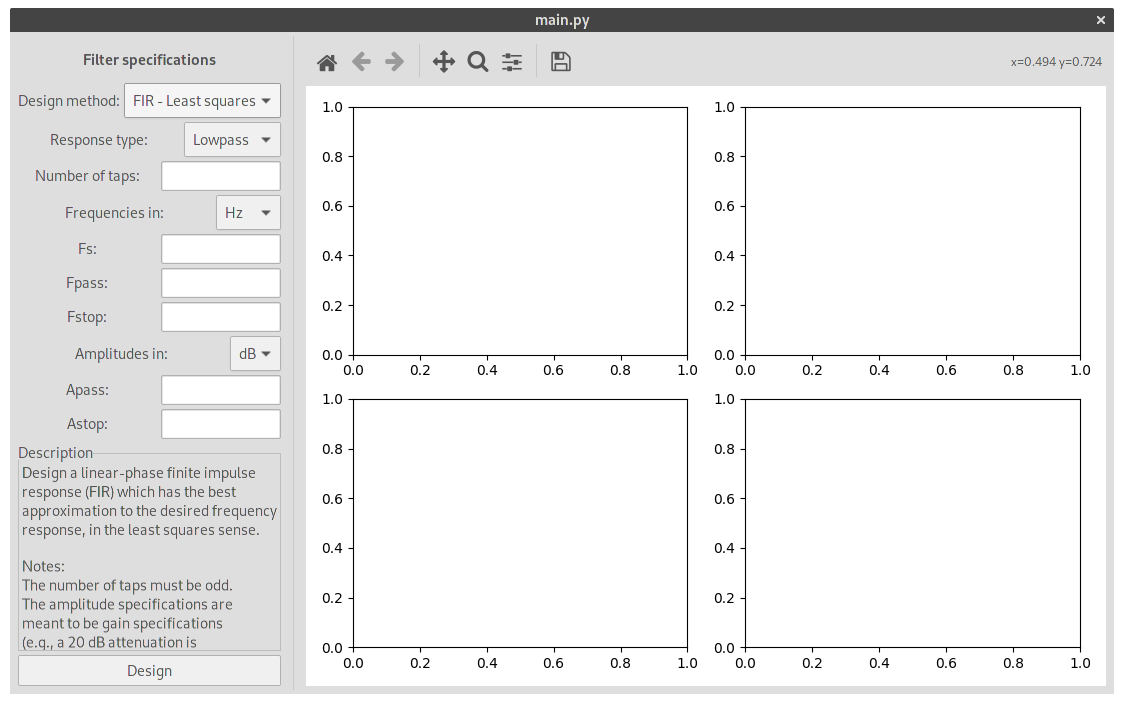
\includegraphics[width=\textwidth]{images/home}
    \label{fig:home}
    \caption*{Fonte: Autoria própria}
  \end{figure}

  A utilização do sistema começa pela escolha de um método de projeto, sendo que cada método possui
  características próprias e até mesmo a interface do sistema muda de acordo para acomodar cada metodologia.
  Ainda, cada método conta com uma breve descrição de seu funcionamento e observações a respeito da forma de
  utilização. Os método de projeto de filtros FIR utilizando o Least Squares e o algoritmo de Remez apresentam
  uma descrição bastante semelhante, porém diferem quanto ao seu princípio de funcionamento: enquanto o Least
  Squares realiza o projeto a partir da minimização do erro quadrático médio \cite{selesnick}, o algoritmo de
  Remez minimiza o erro máximo \cite{mcclellan_parks}.

  Em seguida, faz-se necessária a escolha de um tipo de resposta para o filtro: passa-baixas, passa-altas,
  passa-faixa ou rejeita-faixa. Dependendo do tipo selecionado, serão exibidas entradas correspondentes para a
  correta descrição do filtro desejado. Na sequência, deve-se então fazer a especificação em frequência e em
  amplitude, de acordo com as unidades escolhidas.

  A partir de todas as especificações, ao clicar no botão \textit{Design}, o filtro será projetado e os
  resultados exibidos nos quatro gráficos que apresentam a resposta em frequência (amplitude e fase), polos e
  zeros da função de transferência e a resposta ao impulso do sistema.

  Com um filtro projetado também é habilitada uma opção para exportação do filtro utilizando Pickle
  \cite{pickle}, que permite serializar um objeto do Python em um arquivo que pode ser posteriormente carregado
  e usado em qualquer aplicação Python. O objeto exportado trata-se de uma instância da classe scipy.signal.dlti
  \cite{scipy}, o que permite a filtragem de sinais e a obtenção das diversas características do filtro, tais
  como sua função de transferência, resposta em frequência e resposta ao impulso.

  Nas próximas seções serão detalhados cada um dos métodos de projeto de filtros digitais oferecidos pela
  plataforma, mostrando a forma pela qual as especificações devem ser feitas, bem como os resultados obtidos.
  Cada filtro projetado será também exportado no formato \texttt{.pickle} e utilizado para efetivamente filtrar
  alguns sinais sintetizados programaticamente.

\section{Filtros FIR pelo método Least Squares}
  Para desenvolver um filtro passa-baixas com 55 taps (coeficientes) cuja banda passante vai até 8 kHz, tendo
  ganho unitário (0 dB), e a banda rejeitada iniciando em 9 kHz, com atenuação de 20 dB (um ganho de -20 dB), a
  especificação do filtro seria como mostra a figura \ref{fig:least_squares_specifications}.
  \begin{figure}[H]
    \caption{Especificação de um filtro passa-baixas usando Least Squares}
    \centering
    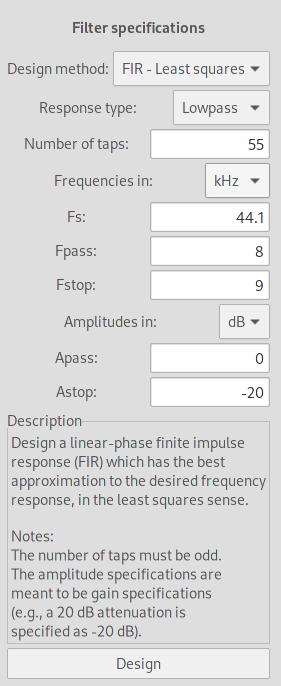
\includegraphics[width=0.4\textwidth]{images/least_squares_specifications}
    \label{fig:least_squares_specifications}
    \caption*{Fonte: Autoria Própria}
  \end{figure}
  
  Os resultados obtidos para estas especificações podem ser visualizados na figura
  \ref{fig:least_squares_results}
  \begin{figure}[H]
    \caption{Resultados do filtro passa-baixas utilizando Least Squares}
    \centering
    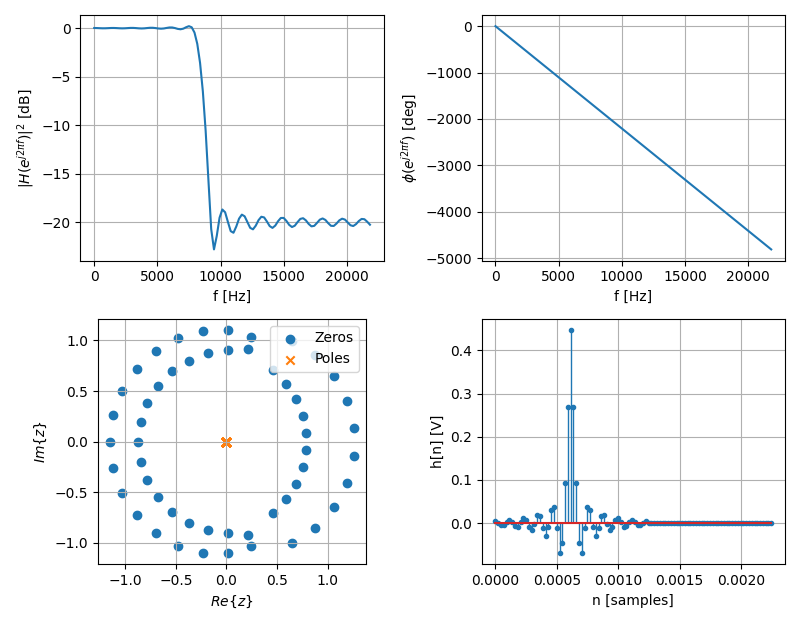
\includegraphics[width=\textwidth]{images/least_squares_results}
    \label{fig:least_squares_results}
    \caption*{Fonte: Autoria Própria}
  \end{figure}

  Exportando o filtro e aplicando-o a um tom de 5 kHz e um de 10kHz, pode-se observar o efeito da filtragem na
  figura \ref{fig:least_squares_tones}.
  \begin{figure}[H]
    \caption{Aplicação do filtro passa-baixas a dois tons}
    \centering
    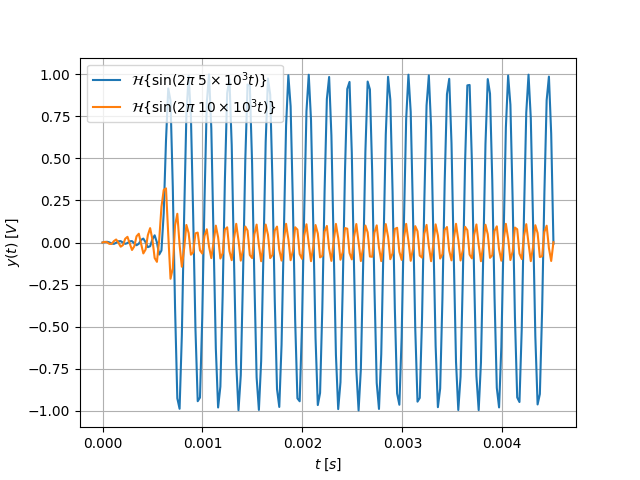
\includegraphics[width=\textwidth]{images/least_squares_tones}
    \label{fig:least_squares_tones}
    \caption*{Fonte: Autoria Própria}
  \end{figure}

  Pode-se perceber que as características desejadas no filtro foram implementadas com sucesso observando sua resposta
  em frequência na figura \ref{fig:least_squares_results}. Quanto aos dois tons sintetizados e filtrados, nota-se que
  o tom de 5 kHz passa praticamente sem sofrer atenuações, enquanto o tom de 10 kHz é reduzido drasticamente. Também
  é possível notar um atraso na saída do filtro, o que é decorrente do tamanho do mesmo (55 coeficientes), sendo
  também esperado quando se leva em conta a fase da resposta em frequência, que apresenta uma inclinação elevada.

\section{Filtros FIR pelo algoritmo de Remez}
  Supondo que se deseje projetar um filtro passa-faixa com 55 taps, cuja banda passante vai de 5 kHz a 15 kHz,
  com ganho unitário (0 dB), e bandas rejeitadas com 1 kHz de transição e atenuações de 20 dB (ganho de -20 dB),
  então a especificação do filtro deve ser feita de acordo com a figura \ref{fig:remez_specifications}.
  \begin{figure}[H]
    \caption{Especificação de um filtro passa-faixa usando o algoritmo de Remez}
    \centering
    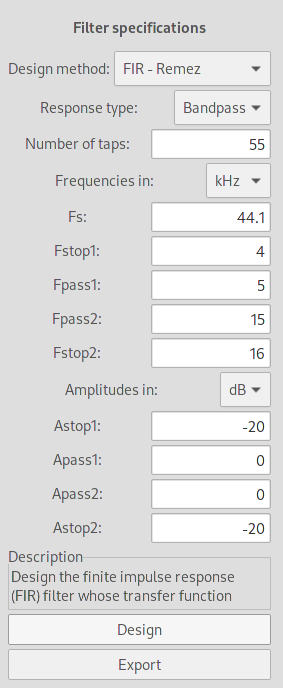
\includegraphics[width=0.4\textwidth]{images/remez_specifications}
    \label{fig:remez_specifications}
    \caption*{Fonte: Autoria Própria}
  \end{figure}

  Para este filtro, os resultados obtidos podem ser vistos na figura \ref{fig:remez_results}.
  \begin{figure}[H]
    \caption{Resultados do filtro passa-faixa utilizando o algoritmo de Remez}
    \centering
    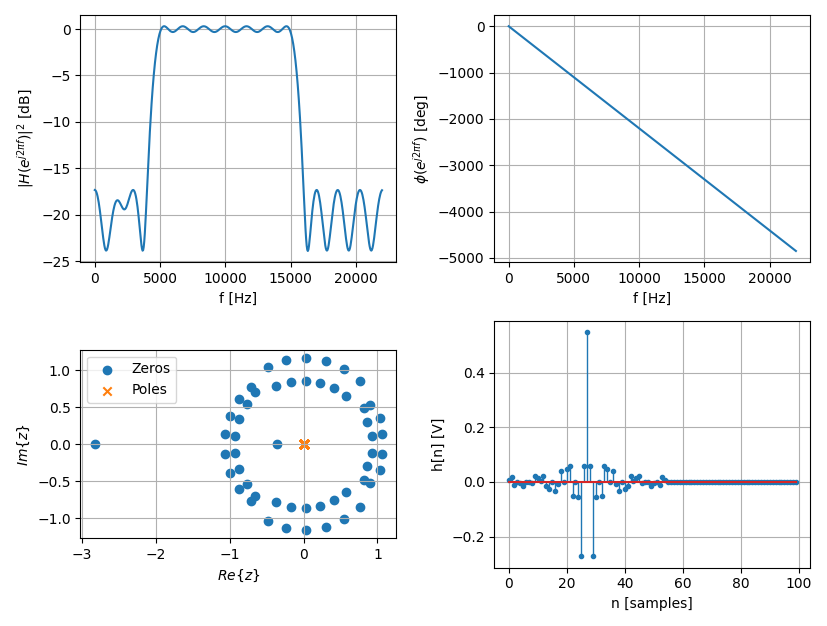
\includegraphics[width=\textwidth]{images/remez_results}
    \label{fig:remez_results}
    \caption*{Fonte: Autoria Própria}
  \end{figure}

  Aqui, fica evidenciado que o filtro projetado está de acordo com as especificações propostas, sendo possível observar
  uma característica específica do algoritmo de Remez: a amplitude da resposta em frequência apresenta \textit{ripples} 
  de igual amplitude, motivo pelo qual estes filtros também são conhecidos como filtros \textit{equiripple}.

  A aplicação do filtro obtido a tons de 2 kHz, 10 kHz e 18 kHz resulta na figura \ref{fig:remez_tones}. Para os três
  tons processados pelo filtro é observada a passagem do tom de 10 kHz, que está dentro da banda passante, enquanto as
  frequências de 2 kHz e 18 kHz são atenuadas.
  \begin{figure}[H]
    \caption{Aplicação do filtro passa-faixa a três tons}
    \centering
    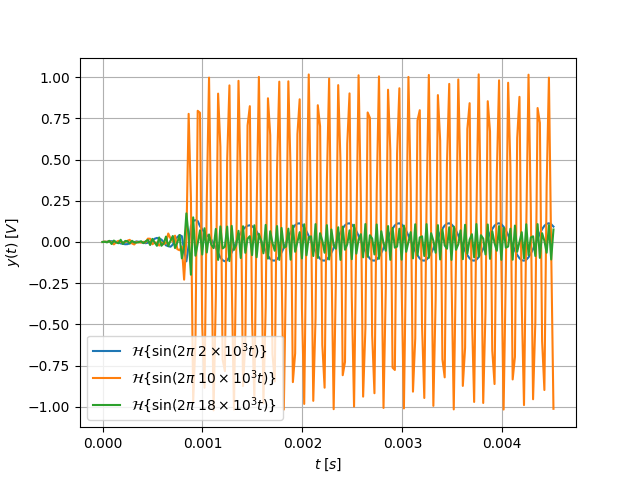
\includegraphics[width=\textwidth]{images/remez_tones}
    \label{fig:remez_tones}
    \caption*{Fonte: Autoria Própria}
  \end{figure}

\section{Filtros IIR}
  Para os filtros IIR, existe a possibilidade de projetar o filtro de acordo com especificações bem definidas
  em relação a resposta desejada bem como de definir a ordem do filtro diretamente. Ao especificar um filtro de
  ordem mínima, será construído um filtro com a mínima ordem necessária para atingir as especificações.

  No caso de um filtro passa-altas Butterworth de ordem 8 com frequência de corte de 8 kHz, a descrição do 
  filtro seria feita como na figura \ref{fig:butter_specifications}.
  \begin{figure}[H]
    \caption{Especificação de um filtro passa-altas de Butterworth}
    \centering
    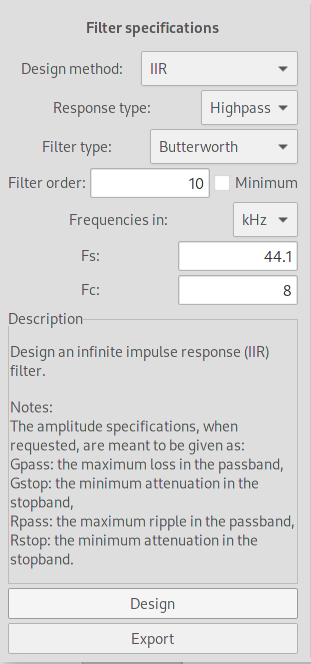
\includegraphics[width=0.4\textwidth]{images/butter_specifications}
    \label{fig:butter_specifications}
    \caption*{Fonte: Autoria Própria}
  \end{figure}

  O filtro projetado apresenta as características exibidas na figura \ref{fig:butter_results}. Como é esperado
  de um filtro Butterworth, tem-se que a amplitude da resposta em frequência do filtro obtido é extremamente
  plana na banda de passagem.
  \begin{figure}[H]
    \caption{Resultados do filtro passa-altas de Butterworth}
    \centering
    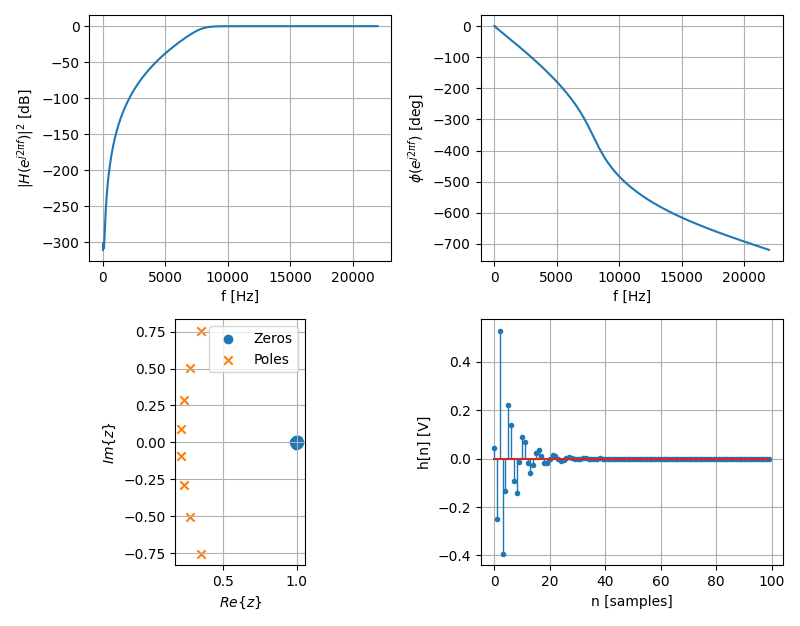
\includegraphics[width=\textwidth]{images/butter_results}
    \label{fig:butter_results}
    \caption*{Fonte: Autoria Própria}
  \end{figure}

  Utilizando o filtro para processar um tom de 4 kHz e um de 12 kHz, obtem-se os resultados mostrados na figura
  \ref{fig:butter_tones}.
  \begin{figure}[H]
    \caption{Aplicação do filtro passa-altas a dois tons}
    \centering
    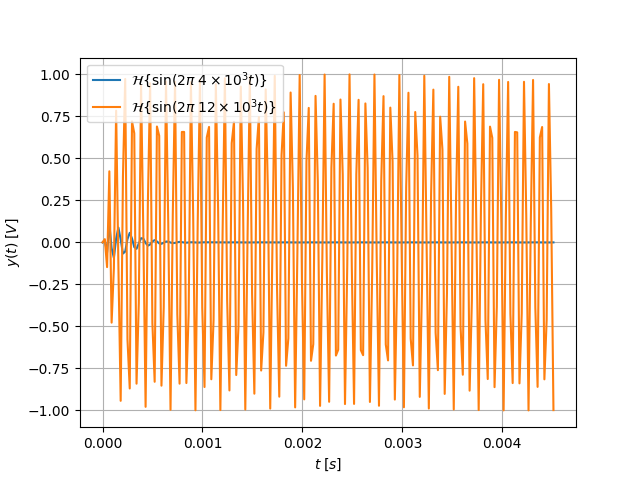
\includegraphics[width=\textwidth]{images/butter_tones}
    \label{fig:butter_tones}
    \caption*{Fonte: Autoria Própria}
  \end{figure}

  Neste caso, a grande atenuação proporcionada pelo filtro faz com que o tom de 4 kHz seja praticamente eliminado
  na saída do mesmo, enquanto o tom de 12 kHz pode passar sem problemas. Vale destacar aqui o pequeno atraso
  introduzido pelo filtro, em relação aos filtros apresentados até então, devido a fase de sua resposta em
  frequência ter uma inclinação consideravelmente menor. Isto se dá em grande parte pela diferença no número
  de coeficientes ou ordem dos filtros considerados.

  Já para um filtro rejeita-faixa de ordem mínima cuja banda rejeitada vai de 4 kHz a 8 kHz, com 500 Hz de faixa
  de transição, uma atenuação de 20 dB na banda rejeitada e atenuação máxima de 3 dB na banda passante, as
  especificações seriam como na figura \ref{fig:cauer_specifications}.
  \begin{figure}[H]
    \caption{Especificação de um filtro rejeita-faixa de Cauer}
    \centering
    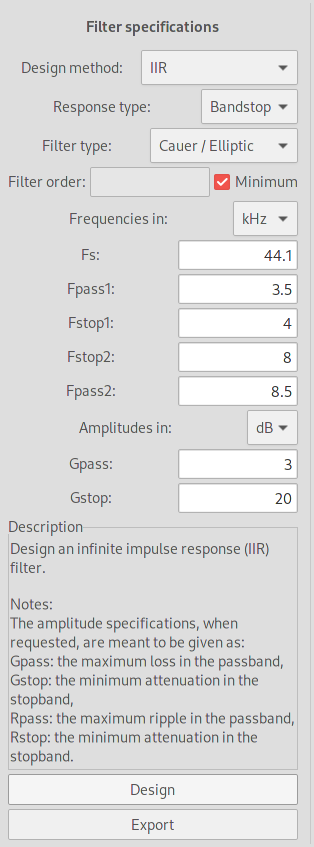
\includegraphics[width=0.4\textwidth]{images/cauer_specifications}
    \label{fig:cauer_specifications}
    \caption*{Fonte: Autoria Própria}
  \end{figure}

  Os resultados obtidos para este filtro podem ser vistos na figura \ref{fig:cauer_results}.
  \begin{figure}[H]
    \caption{Resultados do filtro rejeita-faixa de Cauer}
    \centering
    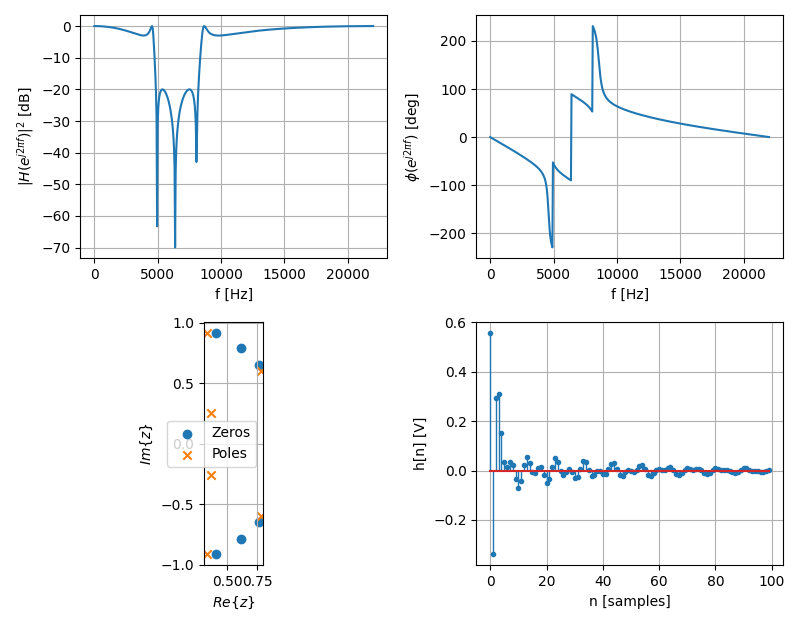
\includegraphics[width=\textwidth]{images/cauer_results}
    \label{fig:cauer_results}
    \caption*{Fonte: Autoria Própria}
  \end{figure}

  É possível observar que as características esperadas pelo filtro de Cauer foram obtidas, sendo respeitadas
  as atenuações mínima de de 20 dB na banda rejeitada e máxima de 3 dB na banda passante. Nota-se ainda que
  a atenuação pode atingir valores bastante elevados, alcançando até 70 dB.

  Aplicando o filtro desenvolvido a tons de 2 kHz, 6 kHz e 10 kHz, obtém-se a figura \ref{fig:cauer_tones}.
  \begin{figure}[H]
    \caption{Aplicação do filtro rejeita-faixa a três tons}
    \centering
    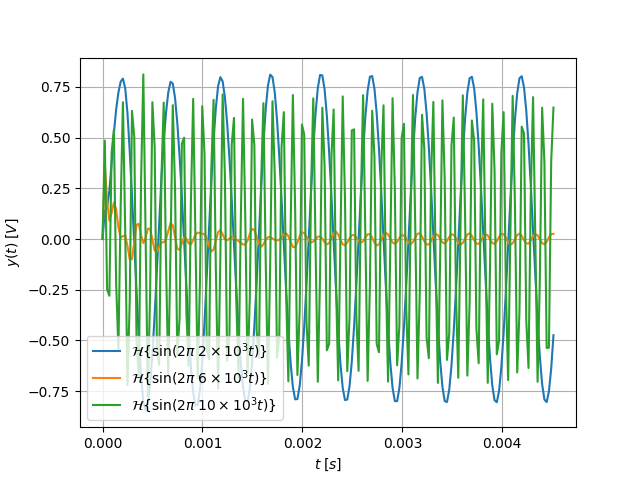
\includegraphics[width=\textwidth]{images/cauer_tones}
    \label{fig:cauer_tones}
    \caption*{Fonte: Autoria Própria}
  \end{figure}

  Os tons processados pelo filtro de Cauer mostram bem a atenuação de 3 dB nas frequências de 2 kHz e 10 kHz,
  resultando em amplitudes de aproximadamente 0.7, enquanto que o tom de 6 kHz foi fortemente atenuado.
  
\chapter{Conclusão}
  Devido à dificuldade de visualização no aprendizado de processamento de sinais, imposta pelo elevado grau de
  abstração envolvido no formalismo matemático da teoria abrangida, foi desenvolvido neste trabalho uma
  ferramenta capaz de realizar o projeto de filtros digitais segundo métodos clássicos da literatura.
  A plataforma construída contempla filtros FIR utilizando os métodos Least Squares e o algoritmo de Remez,
  sendo também tratados os clássicos filtros IIR de Butterworth, Chebyshev I e II, Cauer e Bessel. A aplicação é
  também capaz de fornecer diversos gráficos com intuito de permitir a visualização das principais
  características dos filtros projetados, como sua resposta em frequência, a localização de seus polos e zeros
  no plano complexo e sua resposta ao impulso. Por fim, tem-se ainda a funcionalidade de exportar o filtro
  construído para um arquivo em formato \texttt{.pickle} para a utilização em outras aplicações Python.

  Com a possibilidade de realizar o projeto de filtros digitais por meio de interface gráfica com o usuário,
  a plataforma desenvolvida cumpre com o objetivo de tornar o processo mais prático para o projetista de filtros,
  bem como capacita o aluno com uma ferramenta alternativa durante o aprendizado do tópico de processamento de
  sinais.

\section{Trabalhos futuros}
  Possíveis melhorias foram identificadas para trabalhos futuros, tais quais:

  \begin{itemize}
    \item funcionalidade para permitir a filtragem de sinais diretamente pela plataforma;
    \item adição de outros formatos de exportação (\texttt{.json}, \texttt{.csv}, \texttt{.mat}, etc);
    \item implementação de especificações mais complexas para filtros FIR, como filtros de Hilbert e até mesmo
      filtros multibandas;
    \item possibilidade de edição dos polos e zeros do filtro graficamente;
    \item processamento em tempo real de sinais captados via interface serial com o filtro projetado.
  \end{itemize}

  Ainda, devido a natureza também didática da ferramenta desenvolvida, o \textit{feedback} de alunos a respeito
  de sua utilização pode no futuro apontar para melhorias de \textit{layout} que tornem a plataforma mais
  intuitiva.

\printbibliography[heading=bibnumbered]
\end{document}
